\chapter{The Hot Accretion Flow at 230\,GHz}
\label{ch:xriaf}

Chapter~\ref{ch:xspectral} showed that \sgra{} cannot be fed by a thin disk:
at the measured accretion rate one would outshine it a hundredfold. Its
accretion flow is instead hot, geometrically thick and optically thin over
most of the spectrum, a radiatively inefficient accretion flow (RIAF), and
its emission peaks at the sub-millimetre wavelengths the Event Horizon
Telescope observes. This chapter builds such a flow, traces its 230\,GHz
synchrotron emission with radiative transfer along the Kerr--Schild rays of
Chapter~\ref{ch:xks}, normalises it to the measured flux density, and
compares the result with the EHT's total-intensity \citep{EHT2022} and
polarised \citep{EHT2024pol, EHT2024polint} images of \sgra.

\section{The model}

\paragraph{Plasma.} We adopt the semi-analytic flow that Broderick and
collaborators used to interpret the first millimetre-VLBI data of \sgra{}
\citep{BroderickLoeb2006, Broderick2011}, after \citet{Yuan2003}. With
cylindrical radius $\rho$ and height $z$ (from the Boyer--Lindquist $r$ and
$\theta$), the thermal electrons have
\begin{equation}
n_e = n_0 \left(\frac{\rho}{M}\right)^{-1.1} e^{-z^2/2\rho^2}, \qquad
T_e = T_0 \left(\frac{r}{M}\right)^{-0.84},
\label{eq:riaf}
\end{equation}
with $T_0 = \XRiafTzero$\,K, the value of \citet{BroderickLoeb2006} for their
high-spin model. The field is toroidal and in partial equipartition with the
ions, $B^2/8\pi = \beta^{-1} n_e m_p c^2 r_S/12r$ with $\beta = \XRiafBeta$
\citep{Broderick2011}. The gas circulates at the Keplerian rate of its
cylindrical radius outside the innermost stable orbit and plunges inside it.
On the equator it follows the plunging geodesic with the ISCO's energy and
angular momentum. Off the plane every point takes that plunge's radial and
angular velocity at the same $r$, normalised locally. Only thermal electrons
are modelled. \citet{Broderick2011} attribute roughly 30 per cent of the
1.3\,mm flux in their models to a non-thermal population, which we omit.

\paragraph{Emission and transfer.} The thermal synchrotron emissivity is
the fit of \citet{LeungGammieNoble2011}, as implemented in grmonty
\citep{Dolence2009}:
\begin{equation}
\begin{gathered}
j_\nu = \frac{\sqrt2\,\pi e^2 n_e \nu_s}{3cK_2(1/\Theta_e)}
\left(X^{1/2} + 2^{11/12}X^{1/6}\right)^2 e^{-X^{1/3}}, \\
X = \frac{\nu}{\nu_s}, \qquad
\nu_s = \frac29\,\frac{eB}{2\pi m_e c}\,\Theta_e^2\sin\theta_B ,
\end{gathered}
\end{equation}
where $\Theta_e = kT_e/m_ec^2$ and $\theta_B$ is the angle between the photon
and the field in the fluid frame. Absorption follows from Kirchhoff's law,
$\alpha_\nu = j_\nu/B_\nu(T_e)$. Along a backward ray normalised so the camera
measures unit frequency, the fluid sees $\varepsilon = p\cdot u$, so
$\nu_{\rm f} = \varepsilon\,\nu_{\rm obs}$, and the proper length per affine
step is $\varepsilon\,\Delta\lambda$. For a thermal source the conserved
$I_\nu/\nu^3$ gives the composited solution
\begin{equation}
I_{\rm obs} = \sum_k \frac{B_{\nu_{\rm f}}(T_e)}{\varepsilon^3}
\left(1 - e^{-\Delta\tau_k}\right)e^{-\tau_k},
\qquad \Delta\tau_k = \alpha_{\nu_{\rm f}}\,\varepsilon\,\Delta\lambda\,r_g ,
\label{eq:riaftransfer}
\end{equation}
accumulated from the camera outward. Faraday rotation and conversion are
not modelled.

\paragraph{Normalisation and tests.} The density normalisation is the one
free parameter. It is fitted, by bisection on full images, so that the
230\,GHz flux density equals the EHT benchmark of $\XRiafTarget$\,Jy
\citep{EHT2022}. This gives $n_0 = \XRiafNzero$\,cm$^{-3}$. At the ISCO
the plasma then has $n_e = \XRiafNeIsco$\,cm$^{-3}$, $T_e = \XRiafTeIsco$\,K
and $B = \XRiafBIsco$\,G. Images span $\pm\XRiafHalfWidth\,M$ with
$\XRiafPixels^2$ pixels from a camera at $1000\,M$ (at $\XRiafResLow^2$ pixels
the ring diameter below changes by $\XRiafResD$\,\%), and $|H| \le
\XRiafMaxdH$ along every ray. The test suite (\texttt{test\_riaf.cpp}) checks
four properties:
\begin{itemize}
\item the flow is a unit timelike vector and the field a unit vector
orthogonal to it, inside and outside the ISCO;
\item \eqref{eq:riaftransfer} returns $B_\nu(T)$ for an optically thick
slab and $\sum j\,dl$ for a thin one;
\item $j_\nu$ is linear in $n_e$, vanishes along the field and falls off
exponentially above $\nu_s$;
\item images seen from either side of the equatorial plane are exact
mirror images.
\end{itemize}

\section{The image and the EHT ring}

Figure~\ref{fig:xriaf} shows the result at the EHT viewing geometry
($\astar = 0.94$, $i = 30\degr$). Most of the light comes from a crescent on
the approaching side. It is the direct image of the hot, Doppler-boosted
inner flow and lies \emph{inside} the photon ring, which is visible as a thin
circle at the critical curve. The inner flow's horizon silhouette, the
``inner shadow'' \citep{Chael2021}, appears as the dark spot at the centre.
The peak brightness temperature is $\XRiafTb$\,K, or $\XRiafTbBlur$\,K after
blurring with the $\XRiafBeam\,\muas$ restoring beam of the EHT's CLEAN images.

\begin{figure}
\centering
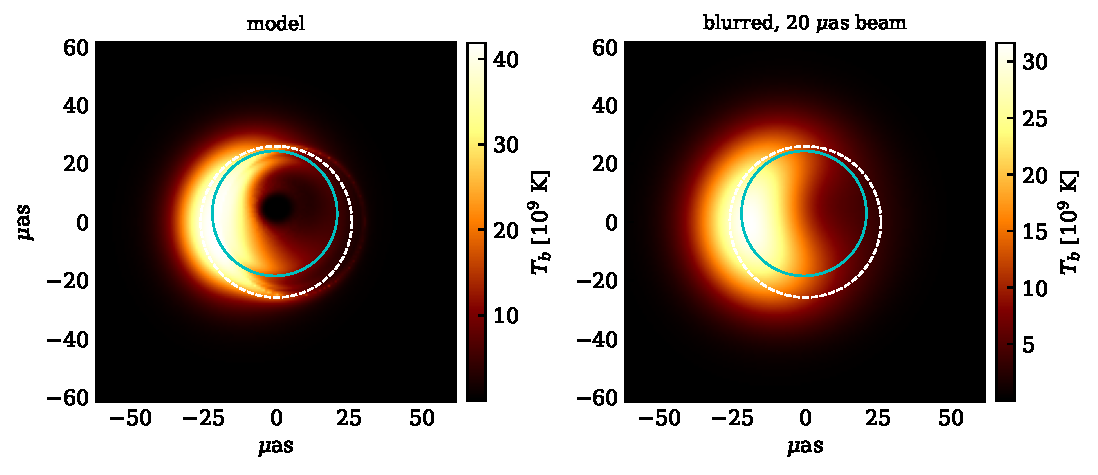
\includegraphics[width=\textwidth]{figures/fig_x_riaf_images.pdf}
\caption{\sgra{} at 230\,GHz in the RIAF model ($\astar = 0.94$, $i =
30\degr$, $n_0$ fitted to $\XRiafTarget$\,Jy), as brightness temperature.
Left: the model image. Right: blurred with the EHT's $\XRiafBeam\,\muas$
restoring beam. Dashed white: the EHT ring diameter, $51.8\,\muas$
\citep{EHT2022}; cyan: the ring measured on the model image.}
\label{fig:xriaf}
\end{figure}

The ring that the brightness peaks trace on the model image, measured as the
EHT's REx procedure does it, has a diameter of $\XRiafDraw\,\muas$ (the
centre minimises the spread of peak radii over 180 position angles). The
EHT measured $51.8\pm2.3\,\muas$. After the $\XRiafBeam\,\muas$ beam the
model's crescent is no longer resolved as a ring: its width exceeds its
diameter, $W/d = \XRiafWdBlur$. The comparison that does not depend on
resolution is the visibility amplitude: blurring multiplies the visibilities
by a Gaussian and leaves their minima where they are. The EHT found its
first and second minima at $|u| \approx 3.0$ and $6.5\,{\rm G}\lambda$,
like a thin ring of about $54\,\muas$ \citep{EHT2022}. Along the position
angles where our model shows a minimum (\XRiafNullPAs\ of 36; the lopsided
crescent fills in the others), the first lies at $\XRiafNullMin$ to
$\XRiafNullMax\,{\rm G}\lambda$. The shortest is equivalent to a thin ring of
$\XRiafThinRing\,\muas$ (Fig.~\ref{fig:xriafvis}).

\begin{figure}
\centering
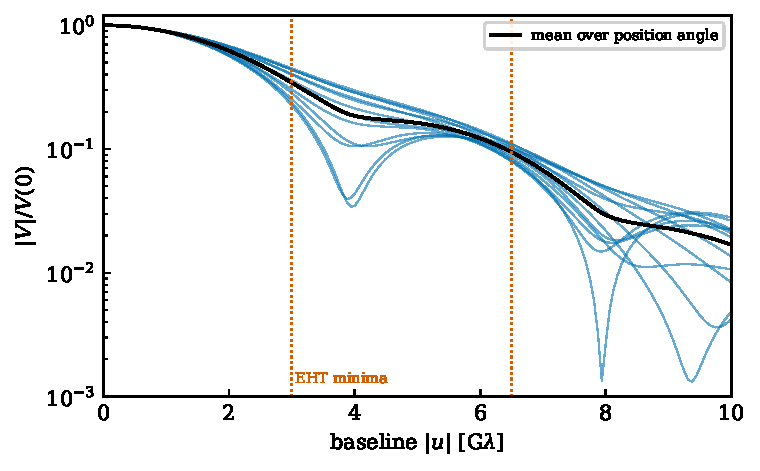
\includegraphics[width=0.78\textwidth]{figures/fig_x_riaf_vis.pdf}
\caption{Visibility amplitudes of the model image of Fig.~\ref{fig:xriaf}
along twelve baseline position angles (blue) and averaged over all (black).
Dotted: the minima of the EHT data \citep{EHT2022}. A beam does not move
these minima.}
\label{fig:xriafvis}
\end{figure}

This model is therefore too compact for \sgra. Its 230\,GHz light is
dominated by the inner flow rather than by the photon ring, and its ring is
$\XRiafRingDeficit$ per cent smaller than the one observed. This is the caveat the thesis
attached to its calibration (the measured ring tracks the critical curve
only as well as the emitting plasma sits on it), made quantitative for one
physical model. The sensitivity runs of Table~\ref{tab:xriaf} show where the
model would have to change. Halving the electron temperature moves the
emission outward and makes the image nearly symmetric: the first minimum
appears along every position angle, at $\XRiafHalfNull\,{\rm G}\lambda$
(a thin ring of $\XRiafHalfThin\,\muas$), and the brightness asymmetry drops
to $\XRiafHalfA$. A nearly face-on view ($i = 10\degr$) gives a ring of
$\XRiafTenD\,\muas$. The field strength barely matters once $n_0$ is
refitted.

\begin{table}
\centering
\caption{The RIAF at 230\,GHz: fitted density normalisation, ring diameter
on the model image, first visibility minimum (shortest over position angles;
in brackets the equivalent thin-ring diameter) and brightness asymmetry after
the $\XRiafBeam\,\muas$ beam, for the reference model and variations
(each refitted to $\XRiafTarget$\,Jy). EHT values from \citet{EHT2022}.}
\label{tab:xriaf}
\small\setlength{\tabcolsep}{4pt}
% AUTO-GENERATED by scripts/make_numbers_ext.py — do not edit by hand.
\begin{tabular}{lcccc}
\toprule
Case & $n_0$ [cm$^{-3}$] & $d$ [$\muas$] & first null [G$\lambda$] ($\muas$) & $A$ \\
\midrule
reference ($T_0$, $\beta = 10$, $i = 30\degr$) & $2.7\times10^{7}$ & 42.8 & 3.90 (40) & 0.33 \\
$T_0/2$ & $1.7\times10^{8}$ & 36.1 & 3.20 (49) & 0.08 \\
$2T_0$ & $9.2\times10^{6}$ & 47.0 & 4.45 (35) & 0.48 \\
$\beta = 3$ & $1.4\times10^{7}$ & 43.3 & 3.85 (41) & 0.35 \\
$\beta = 30$ & $5.1\times10^{7}$ & 42.5 & 3.95 (40) & 0.32 \\
$i = 10\degr$ & $3.1\times10^{7}$ & 49.2 & 3.55 (44) & 0.16 \\
$i = 60\degr$ & $2.3\times10^{7}$ & 27.2 & 4.25 (37) & 0.37 \\
\midrule
EHT 2022 (Paper I) & --- & $51.8 \pm 2.3$ & $\approx 3.0$ ($\approx 54$) & 0.04--0.3 \\
\bottomrule
\end{tabular}

\end{table}

The live renderer offers the same flow as its 230\,GHz band. With identical
parameters and pixel grid it reproduces the fp64 image to $\XRiafGpuFluxDev$\,\%
in total flux, with a correlation of $\XRiafGpuCorr$ and centroids within
$\XRiafGpuCentroidPx$\,pixel (\texttt{compare\_riaf.py}).
Figure~\ref{fig:xbands} shows one camera in the three bands the simulator now
renders.

\begin{figure}
\centering
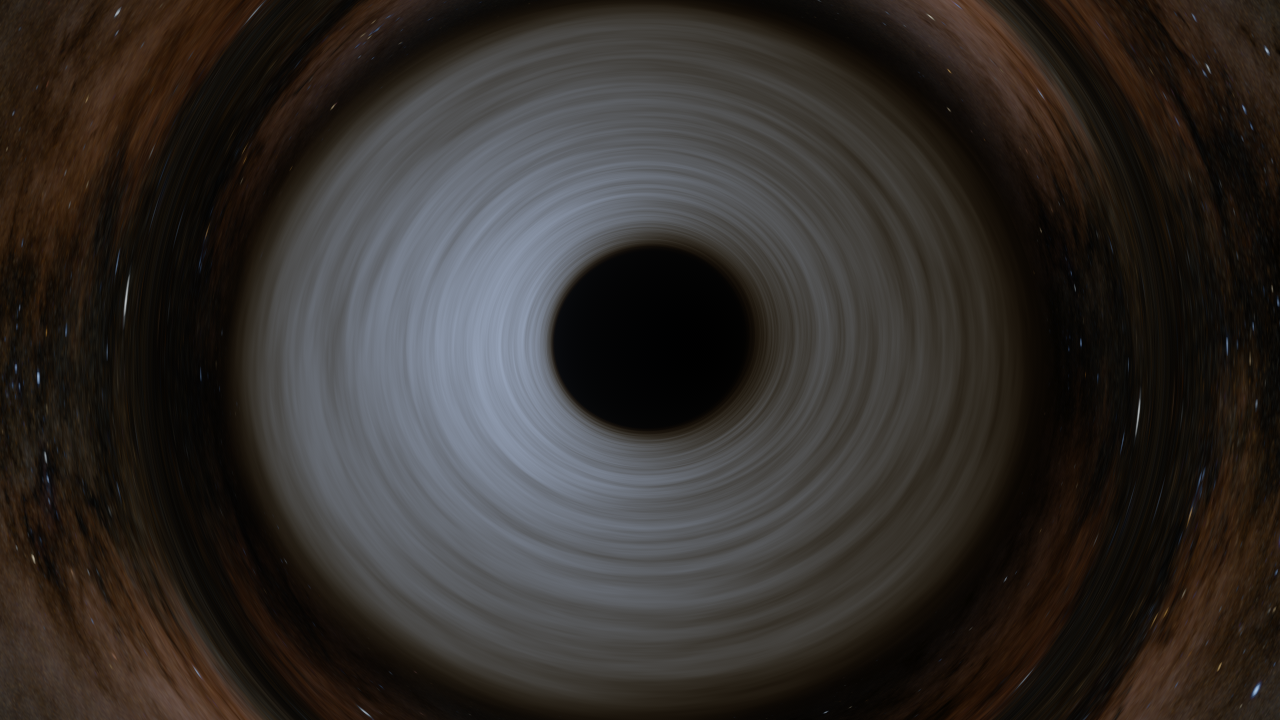
\includegraphics[width=0.32\textwidth]{figures/x_band_visible.png}\hfill
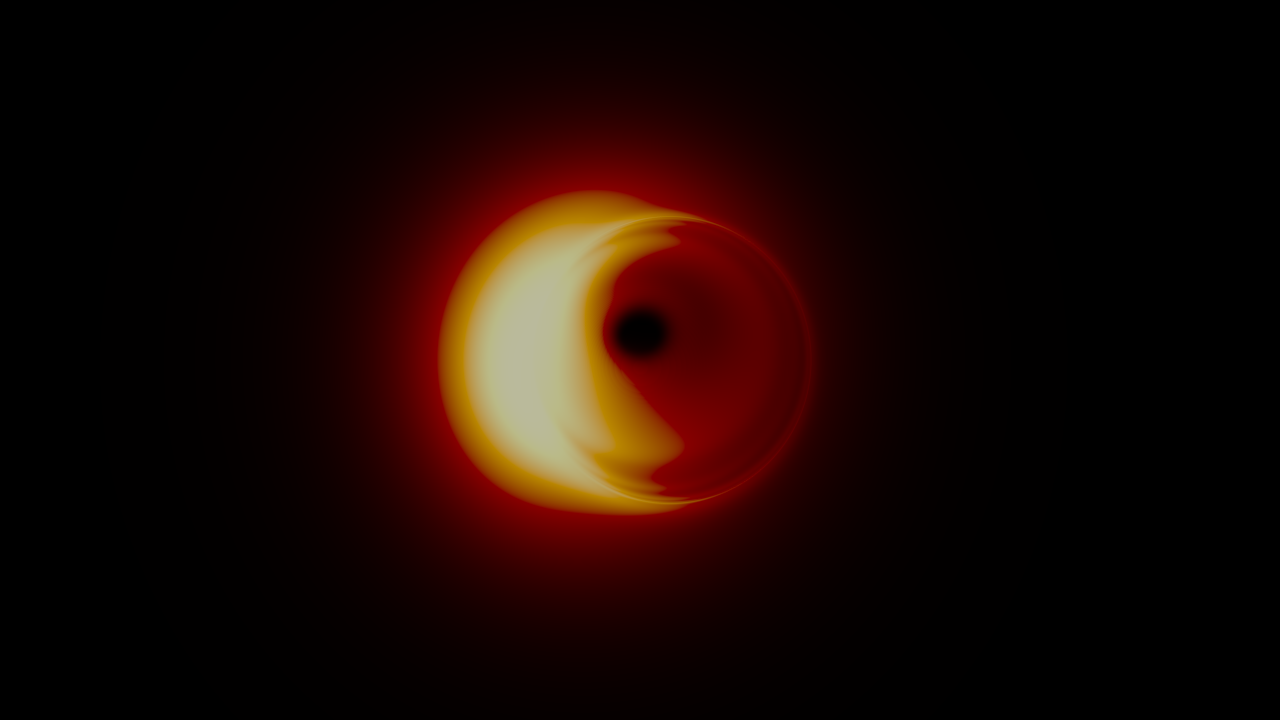
\includegraphics[width=0.32\textwidth]{figures/x_band_230.png}\hfill
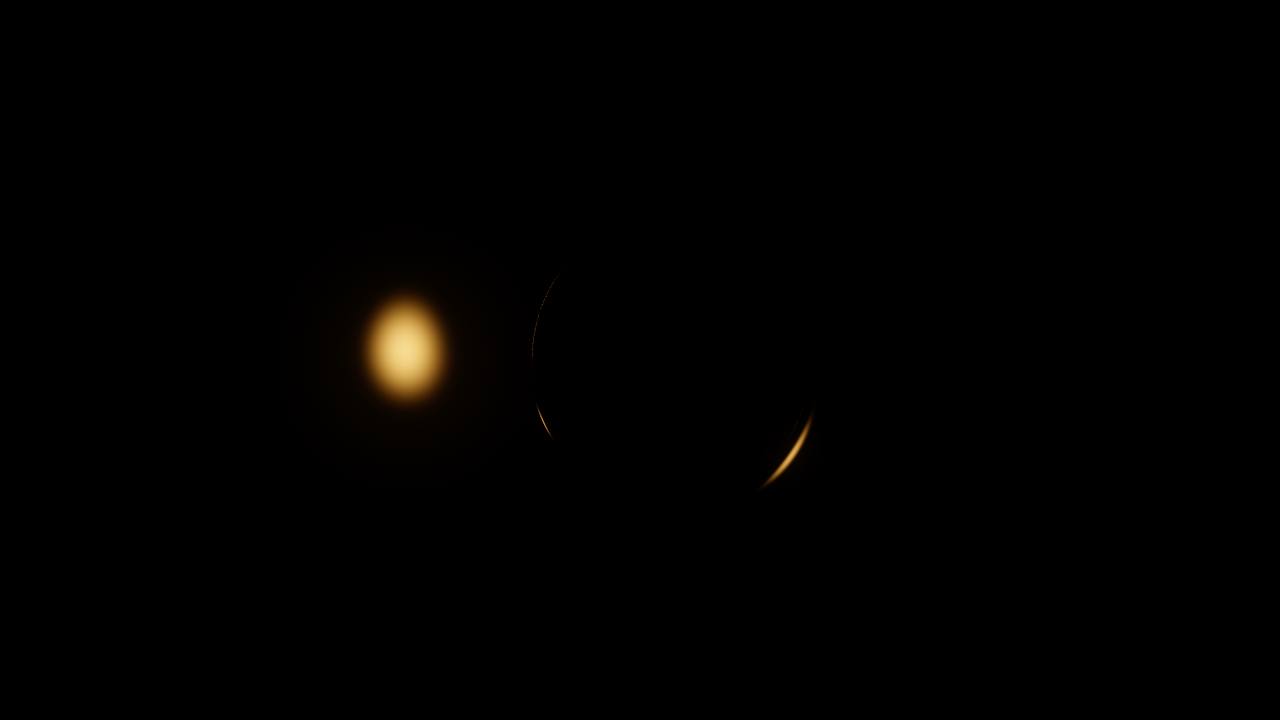
\includegraphics[width=0.32\textwidth]{figures/x_band_kband.png}
\caption{One camera ($i = 30\degr$, $60\,M$), three bands. Left: visible
light, with the hypothetical thin disk of Chapter~\ref{ch:xspectral} and the
lensed Milky Way. Centre: 230\,GHz, the hot accretion flow of this chapter
(brightness temperature, false colour). Right: 2.2\,$\mu$m, a GRAVITY hot
spot (Chapter~\ref{ch:xflares}; false colour). Only the 230\,GHz view shows
\sgra's real quiescent flow.}
\label{fig:xbands}
\end{figure}

\section{Polarisation}
\label{sec:xpol}

Synchrotron light is linearly polarised with its electric vector
perpendicular to both the photon direction and the magnetic field in the
emitting frame, $f^\mu \propto \varepsilon^{\mu\nu\rho\sigma}u_\nu k_\rho
b_\sigma$. Along a Kerr null geodesic the polarisation vector is parallel-
transported, and the \citet{WalkerPenrose1970} constant
\begin{equation}
\kappa = (A - iB)(r - ia\cos\theta), \quad
A = (k^tf^r - k^rf^t) + a\sin^2\theta\,(k^rf^\phi - k^\phi f^r),
\end{equation}
\begin{equation*}
B = \left[(r^2 + a^2)(k^\phi f^\theta - k^\theta f^\phi) - a\,(k^tf^\theta - k^\theta f^t)\right]\sin\theta
\end{equation*}
\citep{ConnorsPiranStark1980, Himwich2020} carries its orientation to the
camera without integrating the transport. At the camera the electric-vector
position angle (EVPA) is the angle $\chi$ in the image plane for which
$\kappa(\cos\chi\,e_1 + \sin\chi\,e_2)$ is a real multiple of the emission
point's $\kappa$, with $e_{1,2}$ the camera's image axes made orthogonal to
the pixel direction.

The tests (\texttt{test\_polarisation.cpp}) cover three properties:
\begin{itemize}
\item $\kappa$ is conserved to $10^{-8}$ when the polarisation vector is
parallel-transported explicitly with the Christoffel symbols along a Kerr
geodesic;
\item a face-on, non-rotating flow with a toroidal field produces a purely
radial EVPA pattern;
\item the views from either side of the equator give complex-conjugate
patterns.
\end{itemize}
Each emitting element contributes Stokes $Q + iU = p_0\,dI\,e^{2i\chi}$ with
a constant intrinsic polarisation fraction $p_0 = \XPolPzero$, an assumption.
Faraday rotation and conversion are omitted.

The EHT summarises the polarisation pattern of a ring by its azimuthal modes
$\beta_m = \sum P e^{-im\phi}/\sum I$ \citep{Palumbo2020}. The phase
$\angle\beta_2$ measures how the EVPAs twist around the ring: 0 for a radial
pattern, $\pm180\degr$ for a toroidal one. It is invariant under rotation of
the image, so the unknown orientation of \sgra's spin on the sky drops out.
Its sign follows the sense in which the flow rotates on the sky. With $p_0$
an assumption, the comparable quantities are $\angle\beta_2$ and
$|\beta_2|/|\beta_1|$, which do not depend on it.

For each field geometry we refit $n_0$ to $\XRiafTarget$\,Jy and view the
flow from $i = 30\degr$ (counter-clockwise on the sky) and $150\degr$
(clockwise, the sense of the GRAVITY flares). Table~\ref{tab:xpol} and
Fig.~\ref{fig:xpol} give the results:
\begin{itemize}
\item \emph{toroidal field} --- the electric vectors point radially,
$|\angle\beta_2| \approx \XPolTorArg\degr$. The EHT measured $\angle\beta_2$
far from zero \citep{EHT2024pol}, so a purely toroidal field is excluded;
\item \emph{radial field} --- a near-toroidal pattern,
$\angle\beta_2 = \XPolRadArgCcw\degr$ (counter-clockwise) or
$\XPolRadArgCw\degr$ (clockwise);
\item \emph{vertical (poloidal) field} --- a spiral,
$\angle\beta_2 = \XPolVerArgCcw\degr$ for counter-clockwise rotation, inside
the EHT's as-observed range of $125\degr$ to $159\degr$, and
$\XPolVerArgCw\degr$ for clockwise rotation, inside the range of $-168\degr$
to $-85\degr$ the EHT obtains after removing a constant (external) Faraday
rotation measure \citep{EHT2024pol}. Its $|\beta_2|/|\beta_1| =
\XPolVerRatio$ compares with the EHT's 1.1--2.1.
\end{itemize}
Only the poloidal field reproduces the observed spiral. That agrees with the
EHT's own interpretation, which favours flows with dynamically important
magnetic fields \citep{EHT2024polint}. Which sign of $\angle\beta_2$ applies
depends on how much of the observed rotation measure is external to the
emitting region, a question this model, which omits Faraday effects, cannot
settle.

\begin{table}
\centering
\caption{Polarisation of the RIAF at 230\,GHz for three field geometries,
seen with counter-clockwise ($i = 30\degr$) and clockwise ($i = 150\degr$)
rotation on the sky: phase of $\beta_2$ on the model and blurred images
(degrees), and on the blurred image $|\beta_2|$, $|\beta_2|/|\beta_1|$, the
resolved $\langle|m|\rangle$ and the net $|m_{\rm net}|$. $|\beta_2|$,
$\langle|m|\rangle$ and $|m_{\rm net}|$ scale with the assumed intrinsic
fraction $p_0 = \XPolPzero$. EHT 90 per cent ranges from \citet{EHT2024pol}.}
\label{tab:xpol}
\footnotesize\setlength{\tabcolsep}{3.5pt}
% AUTO-GENERATED by scripts/make_numbers_ext.py — do not edit by hand.
\begin{tabular}{lrrrrrrr}
\toprule
field & $i$ [deg] & $\angle\beta_2$ & $\angle\beta_2^{\rm blur}$ & $|\beta_2|$ & $|\beta_2|/|\beta_1|$ & $\langle|m|\rangle$ [\%] & $|m_{\rm net}|$ [\%] \\
\midrule
toroidal & 30 & +3 & +1 & 0.43 & 1.5 & 47 & 6.8 \\
toroidal & 150 & -3 & -1 & 0.43 & 1.5 & 47 & 6.8 \\
radial & 30 & -163 & -168 & 0.43 & 2.7 & 44 & 5.4 \\
radial & 150 & +163 & +168 & 0.43 & 2.7 & 44 & 5.4 \\
vertical & 30 & +133 & +135 & 0.27 & 0.8 & 42 & 12.5 \\
vertical & 150 & -133 & -135 & 0.27 & 0.8 & 42 & 12.5 \\
\midrule
EHT 2024, observed & --- & --- & 125 to 159 & 0.14--0.24 & 1.1--2.1 & 24--28 & --- \\
EHT 2024, derotated & --- & --- & $-168$ to $-85$ & & & & \\
\bottomrule
\end{tabular}

\end{table}

\begin{figure}
\centering
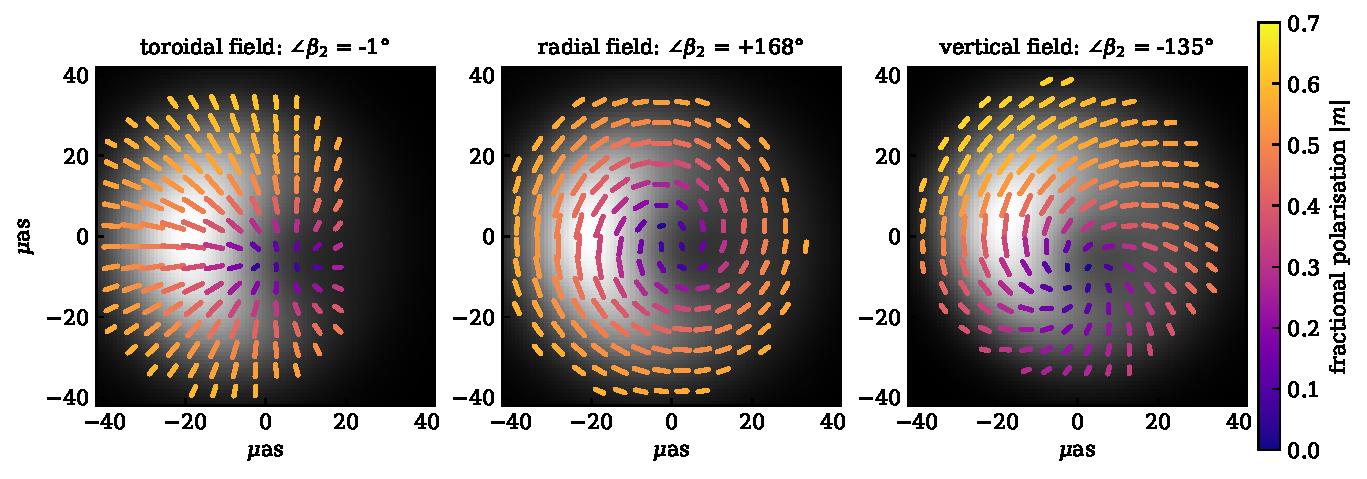
\includegraphics[width=\textwidth]{figures/fig_x_pol.pdf}
\caption{EVPA patterns of the 230\,GHz RIAF for three magnetic-field
geometries, with the flow rotating clockwise on the sky ($i = 150\degr$),
blurred with the EHT beam. Grey: total intensity. Ticks: EVPA, length
proportional to the polarised intensity, colour to the fractional
polarisation. Only the vertical (poloidal) field gives the spiral seen by the
EHT.}
\label{fig:xpol}
\end{figure}
